\documentclass{standalone}
\usepackage{tikz}
\begin{document}

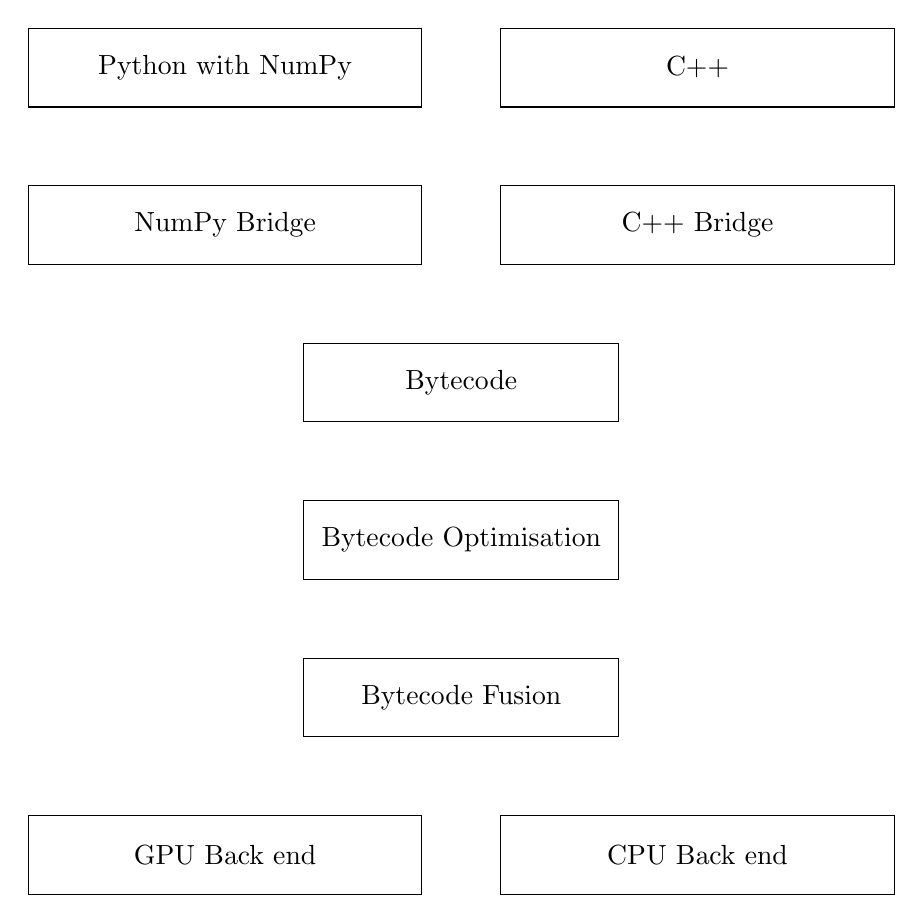
\begin{tikzpicture}
  \draw (1.5,0) rectangle (6.5, 1) node[pos=.5] {Python with NumPy};
  \draw (7.5,0) rectangle (12.5, 1) node[pos=.5] {C++};
  \draw (1.5,-1) rectangle (6.5, -2) node[pos=.5] {NumPy Bridge};
  \draw (7.5,-1) rectangle (12.5, -2) node[pos=.5] {C++ Bridge};

  \draw (5,-3) rectangle (9, -4) node[pos=.5] {Bytecode};
  \draw (5,-5) rectangle (9, -6) node[pos=.5] {Bytecode Optimisation};
  \draw (5,-7) rectangle (9, -8) node[pos=.5] {Bytecode Fusion};

  \draw (1.5,-9) rectangle (6.5, -10) node[pos=.5] {GPU Back end};
  \draw (7.5,-9) rectangle (12.5, -10) node[pos=.5] {CPU Back end};

\end{tikzpicture}

\end{document}
